\section{Measurement of Boosted $H \rightarrow b\bar{b}$} \label{sec:results:procedure}

For the $H \rightarrow b\bar{b}$ process, the observed signal strength is:
%
$$ \mu_{H} = 5.8 \pm 3.1~\mathrm{(stat.)} \pm 1.9~\mathrm{(syst.)} \pm
1.7~\mathrm{(theo.)}\,. $$
%
Using the generator level cross sections ($\sigma_\text{generated}$) from
\Cref{table:data:signal} and the efficiency ($\epsilon$) times acceptance ($A$)
from \Cref{tab:selection:cutflow_higgs} a restricted cross section
($\sigma_\text{restricted}$) for the phase space represented by the presented
analysis selections can be calculated for $H \rightarrow b\bar{b}$ inclusive of
ggF, VBF and VH production mechanisms.  Using the values from
\Cref{tab:results:signal_summary} and multiplying by the observed $\mu_{H}$
gives the observed Higgs boson cross section:
%
$$ \sigma_{H} = 15 \fb \pm 8.2 ~\mathrm{(stat.)} \pm 5.0 ~\mathrm{(syst.)} \pm
4.5 ~\mathrm{(theo.)}\,. $$
%
\begin{table}[!t]
  \centering
  \begin{tabular}{l||c|c|c|c}
     & $ \sigma_\text{generated} (\fb)$ & $\text{n}_\text{SR}$ & $\epsilon \times A$ & $\sigma_\text{restricted} (\fb)$ \\
    \hline
    \hline
    \textbf{ggF}   & 476.3  & 115 & 0.002997 & 1.428 \\
    \textbf{VBF}   & 100.24 & 53  & 0.006319 & 0.6334 \\
    \textbf{WH}    & 8.2914 & 26  & 0.03895  & 0.3230 \\
    \textbf{ZH}    & 4.5178 & 21  & 0.05774  & 0.2609 \\
    \hline
    \textbf{Total} & 589.3  & 215 & 0.04499  & 2.645 \\
  \end{tabular} 
  \caption{Summary of pertinent boosted Higgs boson cross section and selection values in simulation. $\text{n}_\text{SR}$ is the number of simulated Higgs bosons that pass into the SR.}
  \label{tab:results:signal_summary}
\end{table}
%
Given the uncertainties, this result is consistent with the background-only
hypothesis at $1.6\sigma$ with an expected sensitivity of $0.28\sigma$
\cite{Feickert:HiggsCouplings2018}.  This constitutes a measurement of the
boosted Higgs decaying to a bottom quark pair but not a direct observation
which would require $5\sigma$. The result of the combined fit of $V$ + jets and
$H \rightarrow b\bar{b}$ agrees with the Standard Model prediction of $\mu_{H}
= \mu_{V} = 1$, as seen in \Cref{sec:results:contour}.
%
\begin{figure}[!b]
\centering
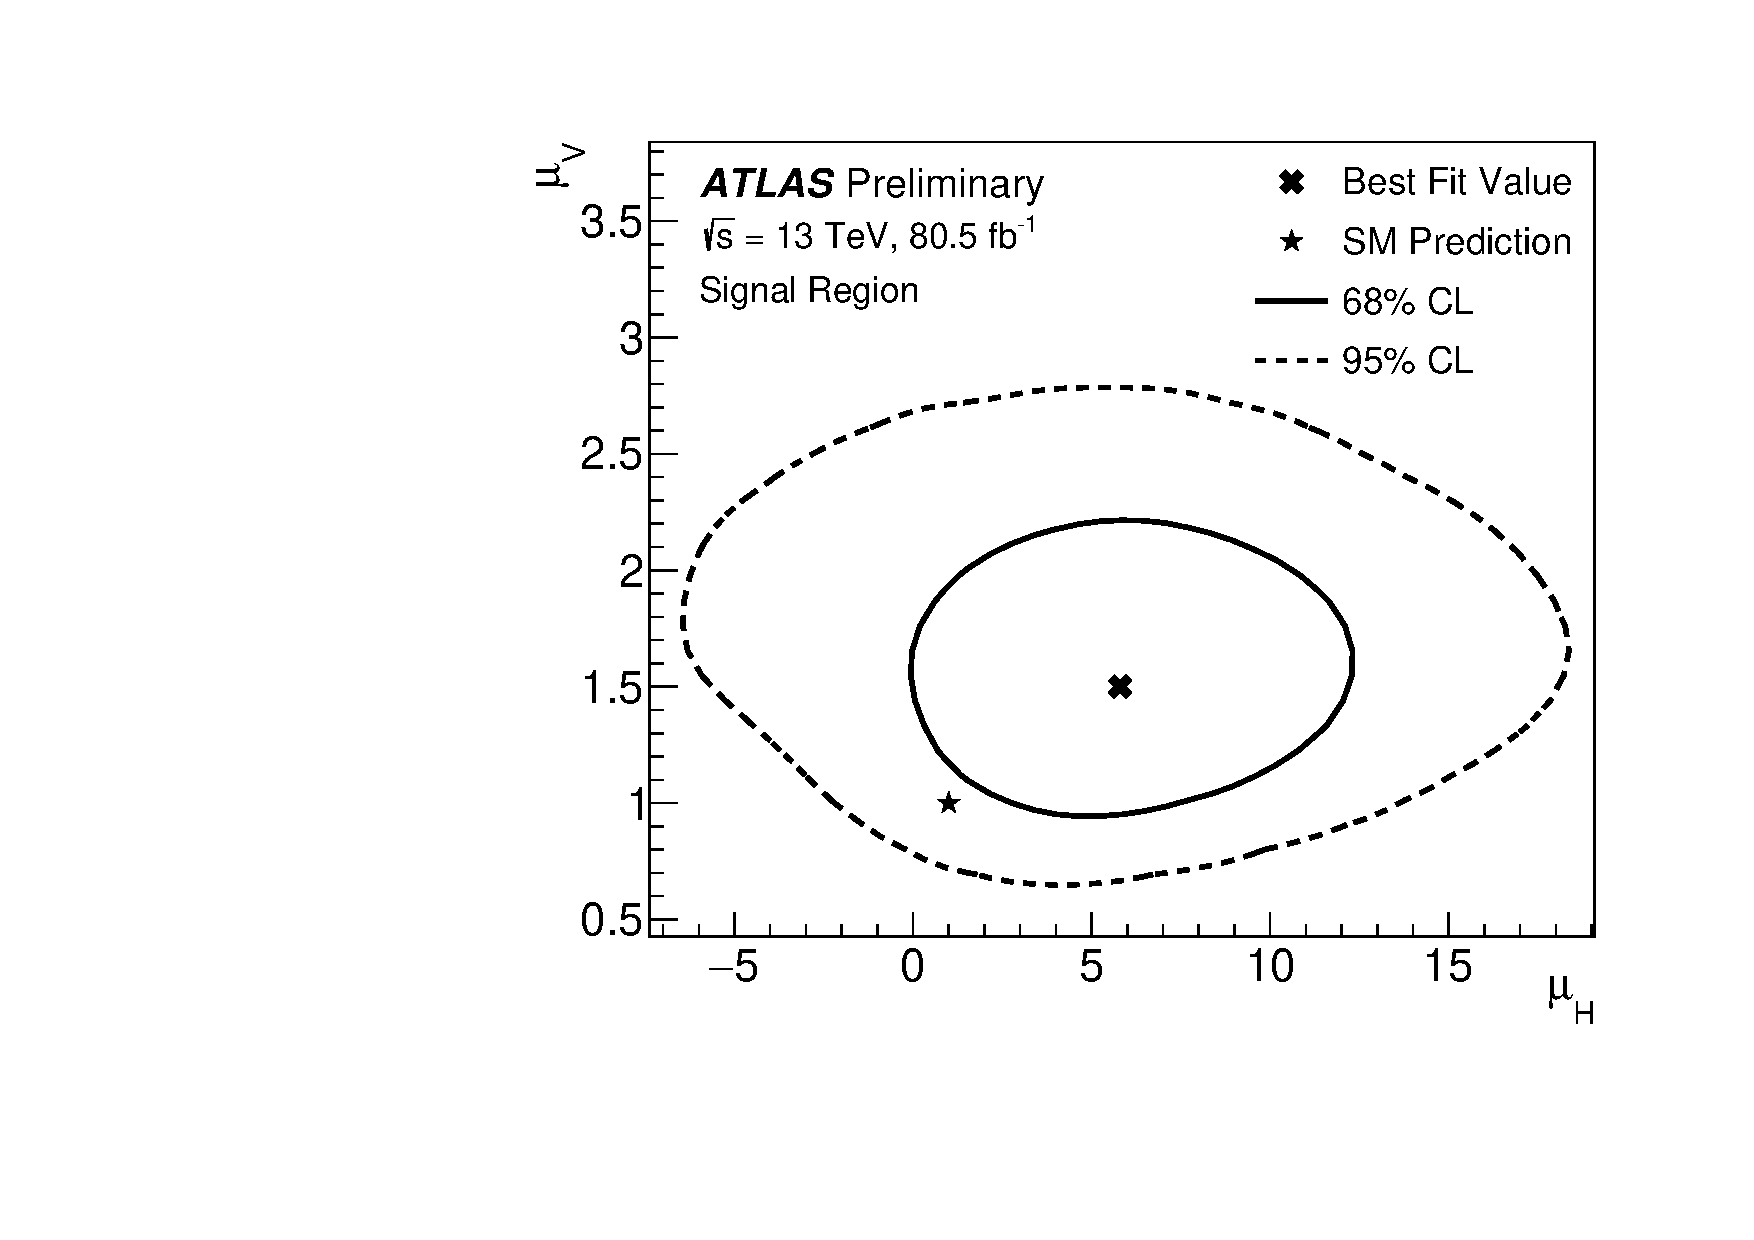
\includegraphics[width=.7\linewidth]{figures/results/contour}
\caption{
Combined marginalized posterior distributions of $\mu_{H}$ and $\mu_{V}$ in the
Signal Region \cite{ATLAS-CONF-2018-052}.  It is seen that the best-fit values for the signal processes
lie within the 68\% Credibility Level ($2\sigma$) of the Standard Model
prediction.}
\label{sec:results:contour}
\end{figure}
